\section{Introduction to systems of ODEs} \label{sec:introtosys}

\LAtt{3.1}

\LO{
\item Classify the order and number of components in a system of differential equations,
\item Verify if a set of functions solves a system of differential equations, and
\item Write a system of differential equations to fit a physical situation.
}

\subsection{Systems}

Often we do not have just one dependent variable and one equation. For instance, we may be looking at multiple populations that are changing over time, or watching how the amount of support for multiple candidates develops leading up to an election. And as we will see, we may end up with systems of several
equations and several dependent variables even if we start with a single
equation.

If we have several dependent variables,
suppose $y_1$, $y_2$, \ldots, $y_n$,
then
we can have a differential equation involving all of them and their
derivatives with respect to one independent variable $x$.
For example, $y_1'' = f(y_1',y_2',y_1,y_2,x)$.
Usually, when we have two dependent variables we have two equations
such as
\begin{align*}
y_1'' & = f_1(y_1',y_2',y_1,y_2,x) , \\
y_2'' & = f_2(y_1',y_2',y_1,y_2,x) ,
\end{align*}
for some functions $f_1$ and $f_2$.  We call the above a
\emph{\myindex{system of differential equations}}.
More precisely, the above is a \emph{\myindex{second order system}}
of ODEs as second
order derivatives appear.
The system
\begin{align*}
x_1' & = g_1(x_1,x_2,x_3,t) , \\
x_2' & = g_2(x_1,x_2,x_3,t) , \\
x_3' & = g_3(x_1,x_2,x_3,t) ,
\end{align*}
is a \emph{\myindex{first order system}}, where $x_1,x_2,x_3$ are
the dependent variables,
and $t$ is the independent variable.

The terminology for systems is essentially the same as for
single equations.
For the system above, a
\emph{solution}\index{solution to a system}
is a set of three functions $x_1(t)$, $x_2(t)$, $x_3(t)$, such that
\begin{align*}
x_1'(t) &= g_1\bigl(x_1(t),x_2(t),x_3(t),t\bigr) , \\
x_2'(t) &= g_2\bigl(x_1(t),x_2(t),x_3(t),t\bigr) , \\
x_3'(t) &= g_3\bigl(x_1(t),x_2(t),x_3(t),t\bigr) .
\end{align*}

In order to verify that something is a solution, we plug the different components
into the solution to see that all of the equations are satisfied; if any one of the equations
is not satisfied, then this set of functions is not a solution.
We usually also have an
\emph{initial condition}\index{initial condition for a system}.  Just like
for single equations we specify $x_1$, $x_2$, and $x_3$ for some fixed $t$.
For example, $x_1(0) = a_1$, $x_2(0) = a_2$, $x_3(0) = a_3$
for some constants $a_1$, $a_2$, and $a_3$.  For the second order system
we would also specify the first derivatives at that same initial time point.
And if we find a solution with constants in it, where by solving for the
constants we find a solution for any initial condition, we call this
solution the \emph{general solution}\index{general solution to a system}.
Best to look at a simple example.

\begin{example}
Sometimes a system is easy to solve
by solving for one variable and then for the second variable.
Take 
the first order system
\begin{align*}
y_1' & = y_1 , \\
y_2' & = y_1 - y_2 ,
\end{align*}
with $y_1$, $y_2$ as the dependent variables and $x$ as the independent
variable.  Consider initial conditions
$y_1(0) = 1$, $y_2(0) = 2$ and solve the initial value problem.
\end{example}

\begin{exampleSol}
We note that $y_1 = C_1 e^x$ is the general solution of the first equation, which we can get because this equation does not involve $y_2$ at all and we can get a solution via our normal first order equation methods.
We then plug this $y_1$ into the second equation
and get the equation $y_2' = C_1e^x - y_2$, which is a linear first order
equation that is easily solved for $y_2$.  By the method of integrating
factor we get
\begin{equation*}
e^x y_2 = \frac{C_1}{2}e^{2x} + C_2 ,
\end{equation*}
or $y_2 = \frac{C_1}{2}e^{x} + C_2e^{-x}$.  The general solution to the system
is, therefore,
\begin{equation*}
y_1 = C_1 e^x , \qquad
y_2 = \frac{C_1}{2}e^{x} + C_2e^{-x} .
\end{equation*}
We solve for $C_1$ and $C_2$ given the initial conditions.
We substitute $x=0$ and find
that $C_1=1$ and $C_2=\nicefrac{3}{2}$.  Thus the solution is
$y_1 = e^x$, and
$y_2 = (\nicefrac{1}{2}) e^x + (\nicefrac{3}{2}) e^{-x}$.
\end{exampleSol}

Generally, we will not be so lucky to be able to solve for
each variable separately as in the 
example above, and we will have to solve for all variables at once.
While we won't generally be able to solve for one variable and then the
next, we will try to salvage as much as possible from this technique.
It will turn out that in a certain sense we will still (try to) solve
a bunch of single equations and put their solutions together.  Let's not
worry right now about how to solve systems yet.

We will mostly consider \emph{\myindex{linear systems}}.  The example
above is an example of a \emph{\myindex{linear first order system}}.
It is linear as none of the dependent variables or their derivatives
appear in nonlinear functions or with powers
higher than one ($x$, $y$, $x'$ and $y'$, constants, and functions of $t$
can appear, but not $xy$ or ${(y')}^2$ or $x^3$).  A more
complicated example of a second order linear system is
\begin{align*}
y_1'' &= e^t y_1' + t^2 y_1 + 5 y_2 + \sin(t), \\
y_2'' &= t y_1'-y_2' + 2 y_1 + \cos(t).
\end{align*}

\subsection{Applications}

Let us consider some simple applications of systems and how to set up the
equations.

\begin{example} \label{sintro:closedbrine-example}
First, we consider salt and brine tanks, but this time water flows
from one to the other and back.  We again consider that the tanks are
well-mixed.

\begin{myfig}
\capstart
\inputpdft{lin-tank-sys}
\caption{A closed system of two brine tanks.\label{sintro:closedbrine}}
\end{myfig}

Suppose we have two tanks, each containing volume $V$ liters of salt brine.
The amount of salt in the first tank is $x_1$ grams, and the amount of salt
in the second tank is $x_2$ grams.  The liquid is perfectly mixed and
flows at the rate $r$ liters per second out of each tank into the other.
See \figurevref{sintro:closedbrine}. 
\end{example}

\begin{exampleSol}
The rate of change of $x_1$,
that is $x_1'$, is the
rate of salt coming in minus the rate going out.
The rate coming in is the
density of the salt in tank 2, that is $\frac{x_2}{V}$, times the rate $r$.
The rate coming out is the
density of the salt in tank 1, that is $\frac{x_1}{V}$, times the rate $r$.
In other words it is
\begin{equation*}
x_1' = \frac{x_2}{V} r - \frac{x_1}{V} r =
\frac{r}{V} x_2 - \frac{r}{V} x_1  = \frac{r}{V} (x_2-x_1).
\end{equation*}
Similarly we find the rate $x_2'$, where the roles of $x_1$ and $x_2$
are reversed.  All in all, the system of ODEs for this problem is
\begin{align*}
x_1' & = \frac{r}{V} (x_2-x_1), \\
x_2' & = \frac{r}{V} (x_1-x_2).
\end{align*}
In this system we cannot solve for $x_1$ or $x_2$ separately.  We must
solve for both $x_1$ and $x_2$ at once, which is intuitively clear since
the amount of salt in one tank affects the amount in the other.
We can't know $x_1$ before we know $x_2$, and vice versa.

We don't yet know how to find all the solutions, but
intuitively we can at least find some solutions.  Suppose we
know that initially the tanks have the same amount of salt.  That is,
we have an initial condition such as $x_1(0)=x_2(0) = C$.  Then clearly the
amount of salt coming and out of each tank is the same, so the amounts are
not changing.  In other words, $x_1 = C$ and $x_2 = C$ (the constant
functions) is a solution:  $x_1' = x_2' = 0$, and
$x_2-x_1 = x_1-x_2 = 0$, so the equations are satisfied.

Let us think about the setup a little bit more without solving it.  Suppose the
initial conditions are $x_1(0) = A$ and $x_2(0) = B$, for two different
constants $A$ and $B$.  Since no salt is coming in or out of this closed system,
the total amount of salt is constant.  That is, $x_1+x_2$ is constant,
and so it equals $A+B$.
Intuitively if $A$ is bigger than $B$, then more salt will flow out of tank
one than into it.  Eventually, after a long time we would then expect
the amount of salt in each tank to equalize. In other words,
the solutions of both $x_1$ and $x_2$ should
tend towards $\frac{A+B}{2}$.  Once you know how to solve systems
you will find out that this really is so.
\end{exampleSol}

\begin{example} \label{sintro:pop-example}
Another example that showcases how systems work is different ways that populations of animals can interact. There are two main interactions that we will consider. The first of these is of two ``competing species.'' The idea here is that there are two species that are trying to coexist in a given area. On their own (without the other species), each one would grow exponentially, but any interaction between the two species is negative for both of them, because they share the types of food and other resources that they need to survive and grow. This gives rise to a system of differential equations of the form
\[ \begin{split}
\frac{dx_1}{dt} &= ax_1 - bx_1x_2 \\
\frac{dx_2}{dt} &= cx_2 - dx_1x_2.
\end{split} \]

In the system here, the coefficient $a$ represents the growth rate of species 1 on it's own, $b$ represents the amount to which the competition for resources affects the growth rate of species 1, $c$ represents the growth rate of species 2, and $d$ represents the magnitude of how the competition affects the growth of species 2. This type of system can also be written to contain logistic growth terms for the two species, resulting in 
\[ \begin{split}
\frac{dx_1}{dt} &= ax_1(K_1 - x_1) - bx_1x_2 \\
\frac{dx_2}{dt} &= cx_2(K_2 - x_2) - dx_1x_2.
\end{split} \]

The other main population model to consider is a ``predator-prey'' interaction. The key components of this model are that the prey population will grow on it's own and the interaction between the two populations is negative, because the presence of predator population will cause the prey population to decrease. On the other hand, the predator population will die off on it's own (without a food source) but the interaction with the prey population causes the predator population to increase. This gives rise to the system of differential equations
\[
\begin{split}
\frac{dx}{dt} &= ax - bxy \\
\frac{dy}{dt} &= -cy + dxy
\end{split}
\]
where $x$ is the prey population and $y$ is the predator population. We will take another look at both of these examples in \sectionref{nlinapps:section} once we have more terminology and techniques to discuss them.
\end{example}

\begin{example} \label{sintro:carts-example}
Let us look at a second order example.
We return to the mass and spring setup, but this time we
consider two masses.

\begin{mywrapfigsimp}{2.0in}{2.3in}
\noindent
\inputpdft{cartsfig}
\end{mywrapfigsimp}
Consider one spring with constant $k$ and two masses $m_1$
and $m_2$.  Think of the masses as carts that 
ride along a straight track with no friction.  Let $x_1$ be the displacement of the first
cart and $x_2$ be the displacement of the second cart.
That is, we put the two
carts somewhere with no tension on the spring, and we mark the position of
the first and second cart and call those the zero positions.
Then $x_1$ measures how far the first cart is from its zero position,
and $x_2$ measures how far the second cart is from its zero position.
The force exerted by the spring on the first cart is
$k(x_2-x_1)$,
since $x_2-x_1$ is how far the string is stretched (or compressed) from
the rest position.  The force exerted on the second cart is the opposite,
thus the same thing with a negative sign.
\myindex{Newton's second law} states that
force equals mass times acceleration.  So the system of equations is
\begin{align*}
m_1 x_1'' & = k(x_2-x_1) , \\
m_2 x_2'' & = - k(x_2-x_1) .
\end{align*}

Again, we cannot solve for the $x_1$ or $x_2$ variable separately.
That we must solve for both $x_1$ and $x_2$ at once
is intuitively clear, since where the first cart goes
depends on exactly where the second cart goes and vice versa.
\end{example}

\subsection{Changing to first order}

Before we talk about how to handle systems, let us note that
in some sense
we need only consider first order systems.
Let us
take an $n^{\text{th}}$ order differential equation
\begin{equation*}
y^{(n)} = F(y^{(n-1)},\ldots,y',y,x)
\end{equation*}
that we would like to convert into a first order system. To do this, we first consider what a first order system would look like. A first order system consists of a set of equations involving the derivative of each of our variables. Let's start with the first variable $u_1= y$. What is the derivative of $y$? Well, it's $y'$, and we don't have a way to represent this in terms of our variables ($u_1$) without any derivatives. So, we add a new variable $u_2$ that we define to be $y'$, which makes the first equation in our system $u_1' = u_2$. 

Well, now we have $u_2$ and we need to determine what its derivative is. Since $u_2 = y'$, $u_2' = y''$. If the order of the equation $n$ is 2, we then have an equation to define what $y''$ is in terms of $y'$, $y$, and $x$, which are $u_2$, $u_1$, and $x$ in our new system. If that's the case, we're done, and if not, we need to define a new variable $u_3 = y''$ so that $u_2' = u_3$. We can continue this process over and over again. 

When do we stop? As illustrated in the previous example with $n=2$, we stop when our derivative $u_n'$ is the $n$th derivative of $y$. This works because our equation tells us exactly what $y^{(n)}$ is in terms of lower order terms, which we have already defined variables for. Thus, we define new variables $u_1, u_2, \ldots, u_n$ and write the system
\begin{align*}
u_1' & = u_2 , \\
u_2' & = u_3 , \\
& ~\, \vdots \\
u_{n-1}' & = u_n , \\
u_n' & = F(u_n,u_{n-1},\ldots,u_2,u_1,x) .
\end{align*}
We solve
this system for $u_1$, $u_2$, \ldots, $u_n$.  Once we have solved
for the $u$'s,
we can discard $u_2$ through $u_n$ and let $y = u_1$.
This $y$ solves the original equation.

\begin{example}
Take $x''' = 2x''+ 8x' + x + t$.  Convert this equation into a first order system. 
\end{example}

\begin{exampleSol}
Letting $u_1 = x$, $u_2 = x'$, $u_3
= x''$, we find the system:
\begin{equation*}
u_1' = u_2, \qquad u_2' = u_3, \qquad u_3' = 2u_3 + 8u_2 + u_1 + t.
\end{equation*}
Since this is a linear system, we can also write this in matrix-vector form, which will be useful for systems that we will analyze later. To do this, we define a vector $\vec{u}$ as
\begin{equation*}
\vec{u} = \begin{bmatrix} u_1 \\ u_2 \\ u_3 \end{bmatrix}.
\end{equation*}
Then, we know that
\begin{equation*}
\vec{u}\ ` = \begin{bmatrix} u_1'\\ u_2'\\ u_3' \end{bmatrix} = \begin{bmatrix} u_2 \\ u_3 \\ 2u_3 + 8u_2 + u_1 + t \end{bmatrix}.
\end{equation*}
We want to rewrite this equation using the vector $\vec{u}$ and a matrix. We can rewrite this last vector as 
\begin{equation*}
\begin{bmatrix} u_1'\\ u_2'\\ u_3' \end{bmatrix} = \begin{bmatrix} u_2 \\ u_3 \\ u_1 + 8u_2 + 2u_3 \end{bmatrix} + \begin{bmatrix}0 \\ 0 \\ t \end{bmatrix}
\end{equation*}
and the right-hand side of this equation can be written as
\begin{equation*}
\vec{u}\ ` =  \begin{bmatrix} u_2 \\ u_3 \\ u_1 + 8u_2 + 2u_3 \end{bmatrix} + \begin{bmatrix}0 \\ 0 \\ t \end{bmatrix} = \begin{bmatrix} 0 & 1 & 0 \\ 0 & 0 & 1 \\ 1 & 8 & 2 \end{bmatrix} \vec{u} + \begin{bmatrix} 0 \\ 0 \\ t \end{bmatrix}. 
\end{equation*}
(Verify that the matrix multiplication works out here!) Therefore, we can write this first order system as
\begin{equation*}
\vec{u}\ ` = \begin{bmatrix} 0 & 1 & 0 \\ 0 & 0 & 1 \\ 1 & 8 & 2 \end{bmatrix} \vec{u} + \begin{bmatrix} 0 \\ 0 \\ t \end{bmatrix}.
\end{equation*}
\end{exampleSol}

Note that if the equation above was non-linear, it would not be possible to write the system version in an appropriate matrix form. It is also important to know how to take initial conditions into account with these problems.

\begin{example}
Convert the initial value problem
\begin{equation*}
x''' = 4e^t x'' - 3(x')^2 + t^2\sin(x) + (t^2 + 1) \qquad x(0) = 2,\ x'(0) = -1,\ x''(0) = 4
\end{equation*}
into a system of first order equations. Simplify the expression as much as possible.
\end{example}

\begin{exampleSol}
We follow the same procedure as the previous example. We define variables $u_1$, $u_2$, $u_3$ as 
\begin{equation*}
u_1 = x \quad u_2 = x' \quad u_3 = x''
\end{equation*}
so that we have the differential equations
\begin{equation*}
u_1' = u_2 \quad u_2' = u_3 \quad u_3' = x''' = 4e^tu_3 - 3u_2^2 + t^2\sin(u_1) + (t^2 + 1)
\end{equation*}
which we can write in vector form as
\begin{equation*}
\vec{u}' = \begin{bmatrix} u_1'\\ u_2'\\ u_3' \end{bmatrix} = \begin{bmatrix} u_2 \\ u_3 \\  4e^tu_3 - 3u_2^2 + t^2\sin(u_1) + (t^2 + 1) \end{bmatrix}.
\end{equation*}
We would now want to try to convert this into matrix form. However, the matrix that we come up with should not depend on $u$ at all. In this case, it would mean that we want to write this equation as
\begin{equation*}
\vec{u}\ ` = \begin{bmatrix} * & * & * \\ * & * & * \\ * & * & * \end{bmatrix} \begin{bmatrix} u_1 \\ u_2 \\ u_3 \end{bmatrix} + \begin{bmatrix} 0 \\ 0 \\ t^2 + 1 \end{bmatrix} 
\end{equation*}
since the extra term needs to be everything that does not depend on $u$. However, while we can determine the first two rows of the matrix, we can not determine the last row. There is no way to pick terms \emph{independent of $u$} to fill in the three stars in the bottom row in order to make the bottom term in the matrix-vector product to equal $4e^tu_3 - 3u_2^2 + t^2\sin(u_1)$. The issue here is that the equation is non-linear; the $u_2^2$ term and the $\sin(u_1)$ term can not be written in this way. Therefore, the best we can do is the vector form, and it can't be written in matrix form.

The last thing we need to deal with is the initial conditions. Since the conditions say that  
\begin{equation*}
x(0) = 2,\ x'(0) = -1,\ x''(0) = 4
\end{equation*}
and we have that $u_1 = x,\ u_2 = x',\ u_3 = x''$, this means that the initial condition should be 
\begin{equation*}
u_1(0) = 2,\ u_2(0) = -1,\ u_3(0) = 4,
\end{equation*}
or
\begin{equation*}
\vec{u}(0) = \begin{bmatrix} 2 \\ -1 \\ 4 \end{bmatrix}.
\end{equation*}
Thus, the full way to write this initial value problem in system form is
\begin{equation*}
\vec{u}' = \begin{bmatrix} u_2 \\ u_3 \\  4e^tu_3 - 3u_2^2 + t^2\sin(u_1) + (t^2 + 1) \end{bmatrix} \qquad \vec{u}(0) = \begin{bmatrix} 2 \\ -1 \\ 4 \end{bmatrix}.
\end{equation*}
\end{exampleSol}

A similar process can be followed for a system of higher order differential
equations.  For example, a system of $k$ differential equations in $k$
unknowns, all of order $n$, can be transformed into a first
order system of $n \times k$
equations and $n \times k$ unknowns.

\begin{example}
Consider the system from the carts example,
\begin{equation*}
m_1 x_1''  = k(x_2-x_1), \qquad m_2 x_2'' = - k(x_2-x_1) .
\end{equation*}
Let $u_1 = x_1$, $u_2 = x_1'$, 
$u_3 = x_2$, $u_4 = x_2'$.  The second order system becomes the
first order system
\begin{equation*}
u_1' = u_2, \qquad
m_1 u_2'  = k(u_3-u_1), \qquad
u_3' = u_4, \qquad
m_2 u_4' = - k(u_3-u_1) .
\end{equation*}
\end{example}

\begin{example}
The idea works in reverse as well.  Consider 
the system
\begin{equation*}
x' = 2y-x , \qquad
y' = x, 
\end{equation*}
where the independent variable is $t$.  We wish to solve for the initial
conditions $x(0) = 1$, $y(0) =0$.
\end{example}

\begin{exampleSol}
If we differentiate the second equation, we get
$y''=x'$.  We know what $x'$ is in terms of $x$ and $y$, and
we know that $x=y'$.  So,
\begin{equation*}
y'' = x' = 2y-x = 2y-y' .
\end{equation*}
We now have the equation $y''+y'-2y = 0$.  We know how to solve this
equation and we find that $y = C_1 e^{-2t} + C_2 e^t$.  Once we have $y$,
we use the equation $y' = x$ to get $x$.
\begin{equation*}
x = y' = -2 C_1 e^{-2t} + C_2 e^t .
\end{equation*}
We solve for the initial conditions $1 = x(0) = -2 C_1 + C_2$
and $0 = y(0) = C_1 + C_2$.  Hence, $C_1 = -C_2$ and $1 = 3C_2$.
So $C_1 = \nicefrac{-1}{3}$ and $C_2 = \nicefrac{1}{3}$.  Our solution is
\begin{equation*}
x = \frac{2e^{-2t} + e^t}{3} ,\qquad
y = \frac{-e^{-2t} + e^t}{3} .
\end{equation*}
\end{exampleSol}

\begin{exercise}
Plug in and check that this really is the solution.
\end{exercise}

It is useful to go back and forth between systems and higher order equations
for other reasons.  For example, software for solving ODE numerically
(approximation) is generally for first order systems.  So to use it,
you have to take whatever ODE you want to solve and convert it to a first
order system.  In fact, it is not very hard
to adapt computer code for the Euler or Runge--Kutta method for first order equations to
handle first
order systems.  We essentially just treat the dependent variable not as
a number but as a vector.  In many mathematical computer languages there is
almost no distinction in syntax.

%In fact, this is what IODE was doing when you had it solve a second order
%equation numerically in the IODE Project III if you have done that project.

\subsection{Autonomous systems and vector fields}

A system where the equations do not depend on the independent variable
is called an \emph{\myindex{autonomous system}}.  For example
the system $y'=2y-x$, $y'=x$ is autonomous as $t$ is the independent
variable but does not appear in the equations.

For autonomous systems we can draw the so-called
\emph{\myindex{direction field}} or \emph{\myindex{vector field}},
a plot similar to a slope field, but
instead of giving a slope at each point, we give a direction (and a
magnitude).  The previous example, $x' = 2y-x$, $y' = x$, says
that at the point $(x,y)$ the direction in which we should travel to satisfy
the equations should be the direction of the vector $( 2y-x, x )$
with the speed equal to the magnitude of this vector.  So we draw
the vector $(2y-x,x)$ at the point $(x,y)$ and we do this for
many points on the $xy$-plane.
For example, at the point $(1,2)$ we draw the vector
$\bigl(2(2)-1,1\bigr) = (3,1)$,
a vector pointing to the right and a little bit up,
while at the point $(2,1)$ we draw the vector $\bigl(2(1)-2,2\bigr) = (0,2)$
a vector that points straight up.
When drawing the vectors, we will scale down
their size to fit many of them on the same direction field.  We are mostly 
interested in their direction and relative size.  See
\figurevref{sintro-vectorfield:fig}.

We can draw a path of the solution in the plane.  Suppose the
solution is given by $x = f(t)$, $y=g(t)$.  We pick an interval
of $t$ (say $0 \leq t \leq 2$ for our example) and plot all the points
$\bigl(f(t),g(t)\bigr)$ for $t$ in the selected range.  The resulting picture is
called the \emph{\myindex{phase portrait}}
(or \myindex{phase plane portrait}).
The particular curve obtained
is called the \emph{\myindex{trajectory}} or \emph{\myindex{solution curve}}.
See an example plot in \figurevref{sintro-vectorfield-sol:fig}.
In the figure the solution starts at $(1,0)$ and travels along the vector field
for a distance of 2 units of $t$.  We solved this system precisely, so
we compute $x(2)$ and $y(2)$ to find
$x(2) \approx 2.475$ and $y(2) \approx 2.457$.  This point corresponds
to the top right end of the plotted solution curve in the figure.

\begin{myfig}
\parbox[t]{3.0in}{
 \capstart
 \diffyincludegraphics{width=3.0in}{width=4.5in}{sintro-vectorfield}
 \caption{The direction field for $x' = 2y-x$, $y' = x$.%
 \label{sintro-vectorfield:fig}}
}
\quad
\parbox[t]{3.0in}{
 \capstart
 \diffyincludegraphics{width=3.0in}{width=4.5in}{sintro-vectorfield-sol}
 \caption{The direction field for $x' = 2y-x$, $y' = x$ with
 the trajectory of the solution starting at $(1,0)$
 for $0 \leq t \leq 2$.%
 \label{sintro-vectorfield-sol:fig}}
}
\end{myfig}


Notice the similarity to the diagrams we drew for autonomous systems in one
dimension.  But note how much more complicated things become when we
allow just one extra dimension.

We can draw phase portraits and trajectories in the $xy$-plane
even if the system is not autonomous.  In this case however we cannot draw
the direction field, since the field changes as $t$ changes.  For
each $t$ we would get a different direction field.

\subsection{Picard's theorem}

Perhaps before going further, let us mention that Picard's theorem on
existence and uniqueness still holds for systems of ODE\@.  Let us restate
this theorem in the setting of systems.  A general first order
system is of the form
\begin{equation} \label{eq:general-system}
\begin{aligned}
x_1' & = F_1(x_1,x_2,\ldots,x_n,t) , \\
x_2' & = F_2(x_1,x_2,\ldots,x_n,t) , \\
& \vdots \\
x_n' & = F_n(x_1,x_2,\ldots,x_n,t) .
\end{aligned}
\end{equation}

\begin{theorem1}[sys:picardthm]{Picard's theorem on existence and uniqueness for systems}%
%
\index{existence and uniqueness for systems}\index{Picard's theorem}
If for every $j=1,2,\ldots,n$ and every
$k = 1,2,\ldots,n$
each $F_j$ is continuous
and the derivative
$\frac{\partial F_j}{\partial x_k}$ exists and is
continuous near some $(x_1^0,x_2^0,\ldots,x_n^0,t^0)$, then a solution to
\eqref{eq:general-system}
subject to the initial condition
$x_1(t^0) = x_1^0$,
$x_2(t^0) = x_2^0$, \ldots,
$x_n(t^0) = x_n^0$
exists (at least for some small interval of $t$'s) and is unique.
\end{theorem1}

That is, a unique solution exists for any initial condition
given that the system is reasonable ($F_j$ and its partial derivatives
in the $x$ variables are continuous).  As for single equations
we may not have a solution for all time $t$, but at least for some 
short period of time.

As we can change any $n$th order ODE into a first order system,
then we notice that this theorem provides also the
existence and uniqueness of solutions for higher order equations
that we have until now not stated explicitly.

\subsection{Exercises}

\begin{exercise}
Verify that $x_1(t) = 2e^{-t} - 2e^{-2t}$, $x_2(t) = e^{-t} - 2e^{-2t}$ solves the system $x_1' = - 2x_2 $, $x_2' = x_1 - 3x_2$.  
\end{exercise}

\begin{exercise}
Verify that $x_1(t) = -2te^{-3t} - 2e^{-3t}$, $x_2(t) = 2te^{-3t} + 3e^{-3t}$ solves the system $x_1' = -5x_1 - 2x_2 $, $x_2' = 2x_1 - x_2$.  
\end{exercise}

\begin{exercise}
Find the general solution of $x_1' = x_2 - x_1 + t$, $x_2' = x_2$.
\end{exercise}

\begin{exercise}
Find the general solution of $x_1' = 3 x_1 - x_2 + e^t$, $x_2' = x_1$.
\end{exercise}

\begin{exercise}\ansMark%
Find the general solution to $y_1' = 3 y_1$, $y_2' = y_1 + y_2$,
$y_3' = y_1 + y_3$.
\end{exercise}
\exsol{%
$y_1 = C_1 e^{3x}$,
$y_2 = y(x) = C_2 e^x+ \frac{C_1}{2} e^{3 x}$,
$y_3 = y(x) = C_3 e^x+ \frac{C_1}{2} e^{3 x}$
}

\begin{exercise}\ansMark%
Solve $y'=2x$, $x'=x+y$, $x(0)=1$, $y(0)=3$.
\end{exercise}
\exsol{%
$x=\frac{5}{3} e^{2t} - \frac{2}{3} e^{-t}$,
$y=\frac{5}{3} e^{2t} + \frac{4}{3} e^{-t}$
}


\begin{exercise}
Write $ay'' + by' + cy = f(x)$
as a first order system of ODEs.
\end{exercise}

\begin{exercise}
Write $x'' + y^2 y' - x^3 = \sin(t)$, 
$y'' + {(x'+y')}^2 -x = 0$ as a first order system of ODEs.
\end{exercise}

\begin{exercise}\ansMark%
Write $x''' = x+t$ as a first order system.
\end{exercise}
\exsol{%
$x_1' = x_2$,
$x_2' = x_3$,
$x_3' = x_1+t$
}

\begin{exercise}\ansMark%
Write $y_1'' + y_1 + y_2 = t$, 
$y_2'' + y_1 - y_2 = t^2$ as a first order system.
\end{exercise}
\exsol{%
$y_3' + y_1 + y_2 = t$, 
$y_4' + y_1 - y_2 = t^2$,
$y_1' = y_3$,
$y_2' = y_4$
}

\begin{exercise}
Write $y^{(4)} - t^2 y''' + e^t y' - (2t+1)y = \cos(t)$ as a first order system.
\end{exercise}

\begin{exercise}
Write the initial value problem 
\[ y'' - 2xy' + 3y = \sin(x) \qquad y(0) = 1,\ y'(0) = -2 \] as an initial value problem for a first order system of ODEs. Make sure to indicate how the initial condition appears as a part of this problem. 
\end{exercise}

\begin{exercise}
Write the initial value problem 
\[ y'' - (y+1)^2 y' - e^{xy} = \cos(x) \qquad y(0) = -1,\ y'(0) = 5 \] as an initial value problem for a first order system of ODEs. Make sure to indicate how the initial condition appears as a part of this problem. Can this be written in matrix form? Why or why not?
\end{exercise}

\begin{exercise}
Write the initial value problem 
\[ y^{(4)} + e^x y'' - 4\cos(x)y' + (x^2 + 1)y = \frac{1}{x-3} \qquad y(0) = 2,\ y'(0) = -3,\ y''(0) = 0,\ y^{(3)}(0) = 1 \] as an initial value problem for a first order system of ODEs. Make sure to indicate how the initial condition appears as a part of this problem. 
\end{exercise}

\begin{exercise}
Suppose two masses on carts on frictionless surface are at 
displacements $x_1$ and $x_2$ as in \examplevref{sintro:carts-example}.
Suppose that a rocket applies force $F$ in the positive direction on cart
$x_1$.  Set up the system of equations.
\end{exercise}

\begin{exercise}\ansMark%
Suppose two masses on carts on frictionless surface are at 
displacements $x_1$ and $x_2$ as in \examplevref{sintro:carts-example}.
Suppose initial displacement is $x_1(0)=x_2(0)=0$, and initial velocity is $x_1'(0) = x_2'(0) = a$ for some number $a$.
Use your intuition
to solve the system, explain your reasoning.
\end{exercise}
\exsol{%
$x_1 = x_2 = at$.  Explanation of the intuition is left to reader.
}

\begin{exercise}
Suppose the tanks are as in 
\examplevref{sintro:closedbrine-example}, starting both at volume $V$,
but now the rate of flow from tank 1 to tank 2 is $r_1$, and
rate of flow from tank 2 to tank one is $r_2$.  In particular,
the volumes will now be changing.  Set up the system of equations.
\end{exercise}

\begin{exercise}\ansMark%
Suppose the tanks are as in 
\examplevref{sintro:closedbrine-example} except that clean water flows in
at the rate $s$ liters per second into tank 1, and brine flows out of tank 2
and into the sewer also at the rate of $s$ liters per second.
\begin{tasks}
\task Draw the picture.
\task Set up the system of equations.
\task Intuitively, what happens as $t$ goes to infinity, explain.
\end{tasks}
\end{exercise}
\exsol{%
a) Left to reader.
\quad b) 
$x_1' = \frac{r}{V} (x_2-x_1)$,
$x_2' = \frac{r}{V} x_1- \frac{r-s}{V}x_2$.
\quad c) As $t$ goes to infinity, both $x_1$ and $x_2$ go to zero,
explanation is left to reader.
}

\begin{exercise}
Match the systems of differential equations below to their corresponding slope fields. Justify.
\begin{equation*}
(i)\ \begin{cases} \frac{dx}{dt} &= x+y \\ \frac{dy}{dt} &= 2y-x \end{cases} \qquad (ii)\ \begin{cases} \frac{dx}{dt} &= x-y \\ \frac{dy}{dt} &= x^2 + y \end{cases} \qquad (iii)\ \begin{cases} \frac{dx}{dt} &= x^2 - y^2 \\ \frac{dy}{dt} &= 3x-1 \end{cases}
\end{equation*}
\begin{tasks}(3)
\task
\parbox[c]{2in}{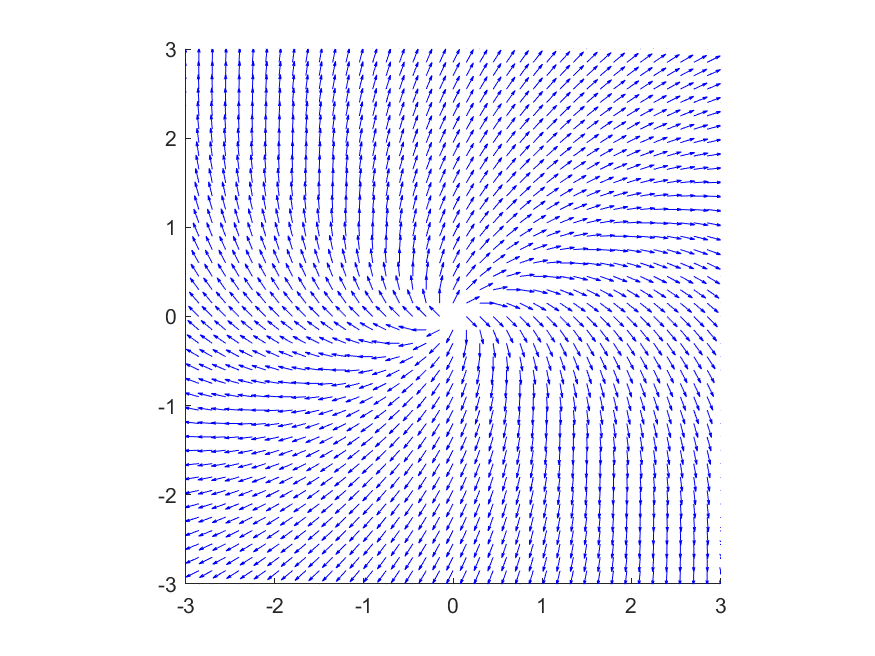
\includegraphics[width=1.75in]{Images/sysslopeEx1_1}}
\task
\parbox[c]{2in}{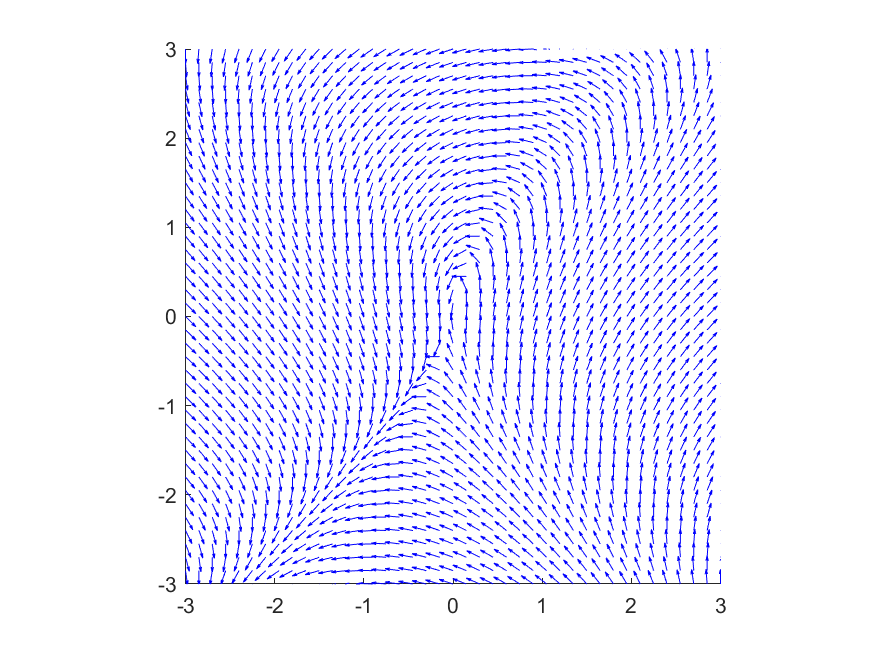
\includegraphics[width=1.75in]{Images/sysslopeEx1_3}}
\task
\parbox[c]{2in}{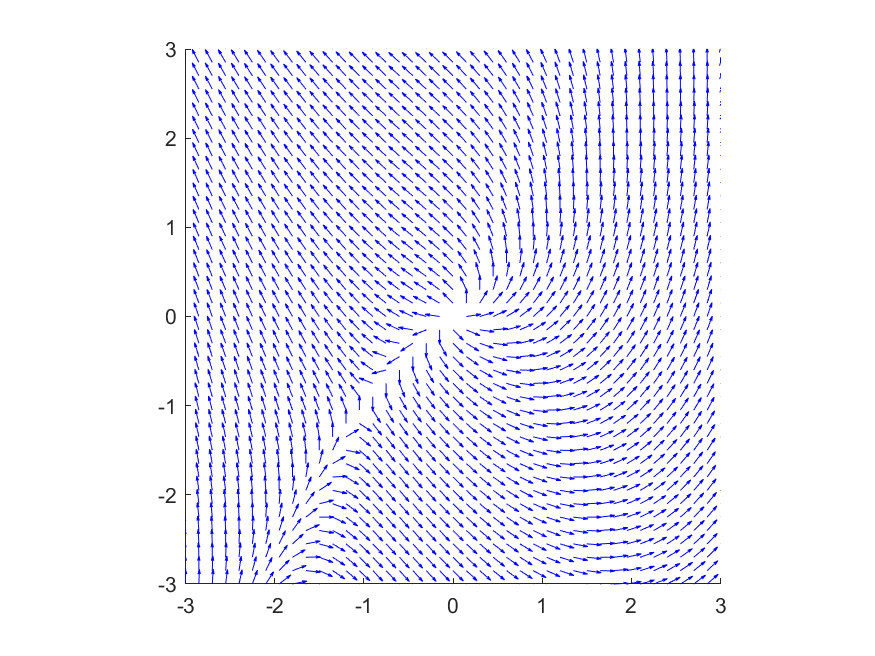
\includegraphics[width=1.75in]{Images/sysslopeEx1_2}}
\end{tasks}
\end{exercise}
\exsol{%
a) (i), \quad
b) (iii), \quad
c) (ii) \quad
Justification left to reader.
}

\begin{exercise}
Match the systems of differential equations below to their corresponding slope fields. Justify.
\begin{equation*}
(i)\ \begin{cases} \frac{dx}{dt} &= 2x+y \\ \frac{dy}{dt} &= y - x^2 \end{cases} \qquad (ii)\ \begin{cases} \frac{dx}{dt} &= x^2 \\ \frac{dy}{dt} &= x-y \end{cases} \qquad (iii)\ \begin{cases} \frac{dx}{dt} &= y+2 \\ \frac{dy}{dt} &= x+y+1 \end{cases}
\end{equation*}
\begin{tasks}(3)
\task
\parbox[c]{2in}{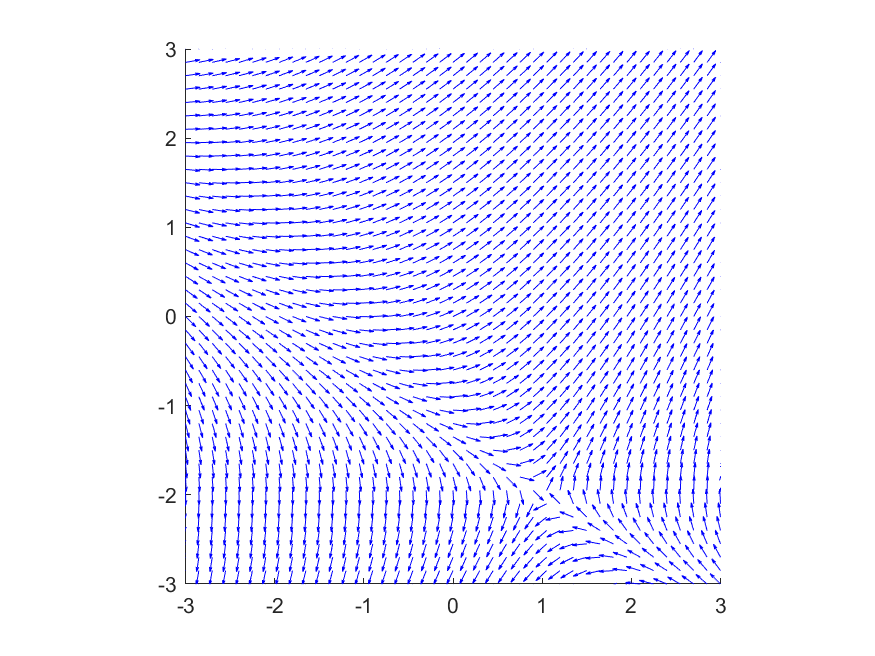
\includegraphics[width=1.75in]{Images/sysslopeEx2_3}}
\task
\parbox[c]{2in}{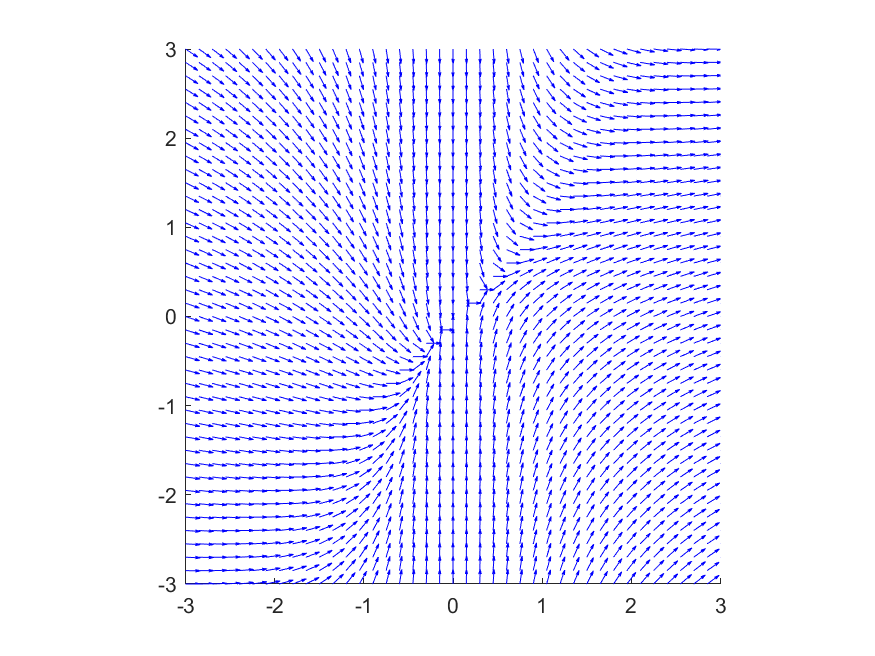
\includegraphics[width=1.75in]{Images/sysslopeEx2_2}}
\task
\parbox[c]{2in}{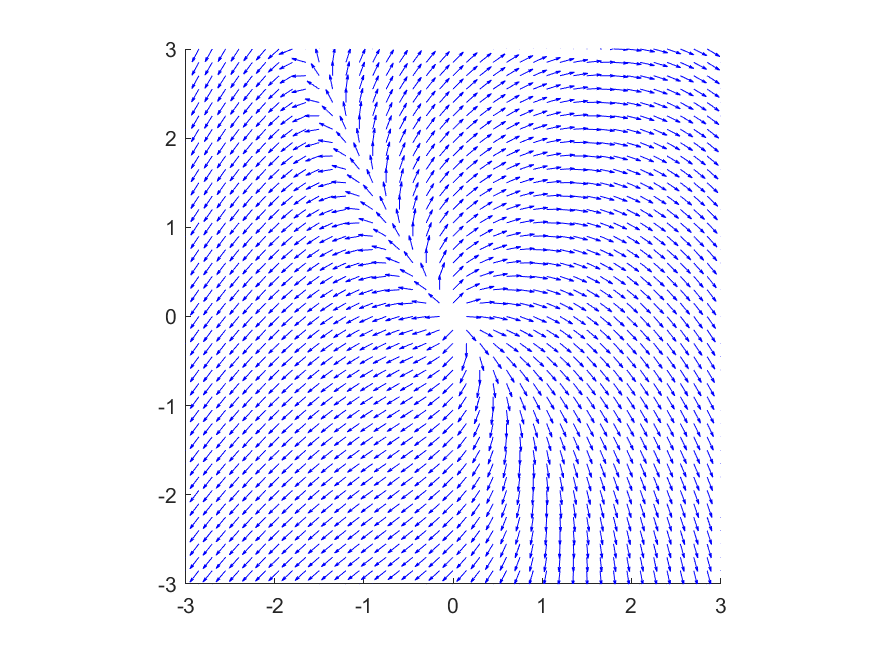
\includegraphics[width=1.75in]{Images/sysslopeEx2_1}}
\end{tasks}
\end{exercise}
\exsol{%
a) (iii), \quad
b) (ii), \quad
c) (i) \quad
Justification left to reader.
}


\setcounter{exercise}{100}


